\vzmstitle{ДОЦЕНТ Е.\,П.~КОСТРЮКОВА}
\vzmsauthor{Воронина (Крейн)}{Т\,.С.}
\vzmsinfo{Fair Lawn, NJ , USA; {\it Tvoronin@yahoo.com} }

\vzmscaption


Евгения Петровна Кострюкова
\textit{(жена С.Г. Крейна и
\linebreak
мать автора заметки~--- ред.)}
работала в должности доцента на химическом факультете ВГУ более 20 лет с 1962~г.
Как оказалось это были самые спокойные, благополучные годы для страны и наиболее плодотворные годы для самого университета и его химического факультета.

Евгения Петровна родилась в сентябре накануне Ок\-тяб\-рь\-с\-кой Революции 1917 года.
Её отец Пётр Кострюков, офицер Русской армии, пропал без вести на полях сражений Первой Мировой войны ещё до рождения дочери. Его жене Ксении Кострюковой, матери Жени, не довелось пожить с горячо любимым мужем сколько-нибудь долгий срок. Практически сразу после венчания его полк отправили на фронт.

Старый уклад жизни рухнул. Ксения в 25 лет от роду, отнюдь не рабоче-крестьянского происхождения, осталась одна,
с дочерью на руках. К счастью, она успела до революции кончить гимназию.
Какое-то время после революции они жили в Кременчуге, где Ксения Юльевна работала учительницей. Жили впроголодь. Однажды в дом ворвались вооружённые люди. Потребовали выдать золото, ценности и хлеб. Ксения Юльевна встретила их с дочерью на руках, распахнула дверцы буфета, где на блюдечке лежала аккуратно завёрнутая четвертушка хлеба. Бандиты хлеб не взяли, а старший подарил ей пачку бритвенных лезвий. Ни он ни она не знали, что с ними делать.

Когда К.\,Ю. уже было за 30, она поступила учиться в Киевский университет на биологический факультет. В это время к ней переехала жить её мать, Антонина Фёдоровна. А.\,Ф. осуждала дочь, говорила, что она уже стара учиться, что надо зарабатывать деньги. Приводила в пример старшую сестру, которая в это время заведовала отделом в Центробанке. К.\,Ю. училась в университете и работала по вечерам на курсах ликвидации неграмотности. Знание языков (в т.ч. латыни) и прекрасная память, а также общая культура обеспечили ей молниеносную карьеру. 10 лет потребовалось К.\,Ю., чтобы закончить институт, защитить кандидатскую, а затем и докторскую диссертации. Ксения Юльевна Кострюкова стала первой женщиной --- доктором наук за всю историю Украины.

Понятно, что заниматься дочерью было некогда.
Женю научили всему, чему положено было учить девочек в российских семьях, две суровые женщины --- её бабушка, Антонина Фёдоровна и её тётя, Вера Юльевна.

Антонина Фёдоровна была воспитанницей Смольного
\linebreak
института благородных девиц.
Она вышла замуж за военврача, родила от него четырёх дочерей. Муж умер рано. Девочки были ещё детьми, их надо было поднимать, выводить в свет, выдавать замуж и А.\,Ф. идёт служить директором женской гимназии. (Интересно, что в этой гимназии преподавал знаменитый поэт Аполлон Майков. А.\,Ф. открывала ежегодный выпускной бал вальсом в паре с Майковым. Пара была на загляденье. А.\,Ф. высокая, стройная (всю жизнь следила за осанкой) и Аполлон внешностью соответствующий имени. Он пил ежедневно и немало. Кто-то написал кляузу. В гимназию пришёл инспектор и посетив урок Майкова написал заключение: <<учитель во время урока зело пьян, но урок ведёт отменно>>.) А.\,Ф. была большой командир. Она могла захлопнуть дверь перед носом Жениного кавалера со словами: <<Мы этого не любим>>. Домашних держала в строгости, руководила ими до конца своих дней, даже уже будучи прикованной к постели.

Вера Юльевна, старшая дочь и сестра К.\,Ю., после гимназии закончила женские Бестужевские курсы. Свободно владела тремя языками. Своих детей не имела. Постоянно жила в Москве, приезжала на лето в Киев помогала сестре вести дом и ухаживать за престарелой матерью. Именно она учила Женю рукоделию, домоводству, готовить еду, хранить вещи, рачительно тратить деньги. В 1914 году, как и многие молодые женщины её сословия, пошла волонтёром в госпиталь, ухаживать за поступающими с фронтов ранеными. В. Ю. была необыкновенно педантична и требовательна к себе. В первые годы Советской власти сделала карьеру. О ней даже писали в газете <<Известия>>, что она, женщина, в течение 12 лет руководит отделом из одних мужчин в Центробанке и не допустила ни разу ни одной ошибки. Впоследствии правда осталась почти без средств к существованию.

Все в семье очень любили Женю, но в силу
обстоя-\linebreak тельств
их жизни совершенно не баловали.
Женя росла прилежной, вдумчивой и не доставляла слишком много хлопот родным. Слушалась бабушку. К тёте Вере относилась с большой нежностью и теплотой, переписывалась с ней потом всю жизнь, поддерживала её, помогала материально. К.\,Ю. Женя просто боготворила, хотя почти совсем не видела. Любила ходить на её доклады, восхищалась эрудицией, находчивостью, умением <<выпускать коготки>> в дискуссии с оппонентами.

Женя начала работать с 15 лет. Испугавшись за мать, она ушла из школы в 8 классе и устроилась на работу учительницей физкультуры. В то время у К.\,Ю. была проблема с рукой. Её парализовало и все боялись, что она не сможет больше работать. Всё обошлось, К.\,Ю. вылечилась и проработала до 83 лет. Женя пошла на подготовительные курсы и поступила учиться в университет на физико-химическое отделение, которое закончила с отличием. По окончании университета работала одновременно м.н.с. в отделе Неорганической химии лаборатории Сорбционные процессы АН \linebreak УССР и учителем в школе.

Вышла замуж по обоюдной любви. Родила сына, Серёжу. Серёжа был здоровым, очень симпатичным ребёнком. Семья мужа приняла Женю хорошо. Первая невестка, первый внук от старшего сыны. Бабушка с дедушкой очень любили гулять с Серёжей --- прохожие часто останавливались полюбоваться красивым мальчиком. Потом война. Эвакуация на Урал. Муж погиб в первый же год. В эвакуации их преследовали болезни. У Серёжи одна детская болезнь следовала за другой. В два с половиной года он перестал говорить. То что удалось его выходить все считали чудом. Ей потребовался не один год лечения, чтобы восстановить своё здоровье. Для Серёжи пагубные последствия этого периода особенно сильно сказались в его зрелые годы. Он много болел и пережил свою мать всего на несколько лет.

С большим трудом ей удалось вернуться из эвакуации в Киев. Работала ассистентом на кафедре Общей и Неорганической химии в Киевском Медицинском Институте, вела практические занятия по курсу физической химии, качественному и количественному анализу. Поступила в аспирантуру в Институт Физической Химии АН УССР.

Вышла замуж за Селима Григорьевича Крейна и родила дочь, Таню. Таня это я. Мои родители познакомились случайно, в поезде, вместе играли в карты. Они помнили друг друга по Киевскому университету. Папа помнил старшекурсницу, химичку, красавицу, замечательную спортсменку. Она выступала на соревнованиях по художественной гимнастике и плаванию. Мама помнила сумасшедшего мальчишку, первокурсника, на костылях победно скользящего по натёртому паркету университетских коридоров. Сам разбежаться не мог, разогнаться ему помогали товарищи. Впоследствии неправильно сросшуюся в колене ногу (результат детской травмы) врачи смогли вытянуть и у папы на всю жизнь осталась только лёгкая хромота.

\begin{center}
{\centering
Братья Крейн
\\
{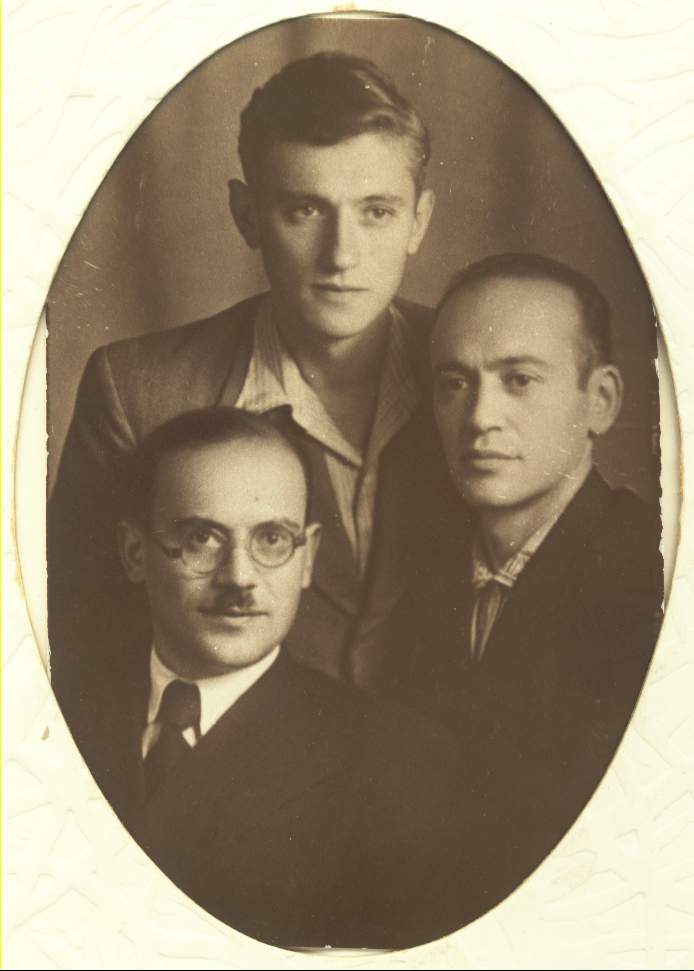
\includegraphics[width=5cm]{hist/MarkSelimMIkhail02Kreinfamily05.jpg}}
\\
Cлева направо~--- Марк Григорьевич, Селим Григорьевич и Михаил Григорьевич
\\
{\centering{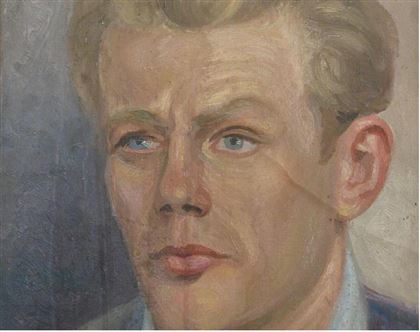
\includegraphics[width=5cm]{hist/portrait.jpg}}}
\\
Портрет учителя \textit{(написал Крейн Дмитрий Григорьевич)}
}
\end{center}
%\hspace{2em}



Женя сомневалась, нужно ли ей выходить за него замуж. Она вдова, у неё уже сын. Он молодой --- ей ровесник, видимо талантливый математик --- в свои 28 уже докторант, красавец, не обременён семьёй. Отец был настойчив. Он решил, что нашёл то, что ему необходимо. Близкие и друзья были озабочены поисками для него жены. Выбор был большой. С.\,Г. выбрал Женю и оказался прав. Они прожили всю жизнь. Всегда хотели быть вместе. И даже когда приблизилась старость и немощь, были готовы на все, лишь бы не разлучаться.

С.\,Г. пришлось сильно постараться, чтобы вписаться в женское царство семьи Жени. Возможно время было такое, или Антонина Фёдоровна задала тон, но мужчин в семье не жаловали. Она и её дочери достаточно красивые, умные, трудолюбивые, все остались без мужей в молодом возрасте, не делали попыток пристроиться, предпочли карабкаться по социальной лестнице самостоятельно. Считалось, что мужчина становится препятствием на пути самореализации женщины в обществе. Феминизм С.\,Г. не испугал. Естественно бастион пал.

Однако их брак~--- недобитой дворянки, аристократки и не разоблачённого до конца космополита,
с карьерной и идейно-полити\-ческой точки зрения имел весьма сомнительные перспективы в то время.
Моя бабушка, К.\,Ю., признавала только положительную коннотацию слова космополит~--- в значении противоположном националист. Она учила меня, что каждый человек, если он претендует, чтобы его считали интеллигентным человеком, должен быть космополитом. Развёрнутую в стране кампанию по борьбе с космополитизмом считала глупостью, желанием выслужиться перед начальством, недостойным способом конкурировать. Отец понимал действия властей до конца. Шла подготовка к окончательному решению еврейского вопроса, в подражание \linebreak Гитлеру. Необходимо было уехать из Киева. С.\,Г. взял в министерстве направление на работу в Воронежский Лесотехнический институт. Здесь требовались квалифицированные преподаватели математики и химии.

Воронеж \ldots

Воронеж стал для семьи второй родиной. При выборе места жительства среди прочего, очень важное значение имело соображение --- понравится ли жене. С.\,Г. говорил, что приехал, посмотрел --- лес, речка, --- решил, понравится. Дело в том, что у его жены было очень сильно развито эстетическое чувство. Ей было не все равно в каком месте жить, в каком здании работать.

Семья получила квартиру в деревянном, двухэтажном доме на улице Морозова, последней улицы города, недалеко от ЛТИ. За домом и сейчас настоящий лес. Из удобств в доме был только свет. То есть вода из колонки посреди улицы, для обогрева в каждой комнате --- топить печь. Конечно это был большой контраст их квартире с горячей водой, газом в историческом, засаженном липами и каштанами центре Киева.
Как же сильно мы все любили этот дом! Мы прожили там с 1954 г. по 1966 г. Жили бы там всю жизнь, но деревянные перекрытия съел жучок. Родители за свой счёт провели в дом воду, сделали паровое отопление, поставили ванну, туалет. Мама разбила вокруг дома садик. В то время как соседи сажали картошку, капусту, помидоры, мама посадила берёзки, рябинки, жасмин, цветы.

Е.\,П. очень любила природу. Знала правильные названия всех растений с детства (переняла у К.\,Ю., когда сопровождала её на уроках на открытом воздухе). А мы любили мамин просветлённый взгляд, сияющее светом лицо во время наших прогулок по окрестностям. Благодаря ей муж и мы, дети, научились наслаждаться незатейливой красотой природы нашей средней полосы, впитывать и различать различные запахи луга, леса, реки, болот.
Е.\,П. хотела остаться жить в районе СХИ и они купили кооператив на ул. Тимирязева, где и прожили всю оставшуюся жизнь.

Только по прошествии более 10 лет мы узнали, что с районом СХИ связано имя нашего родственника Н.\,П.~Макарова. Это муж Аллы Юльевны, ещё одной маминой тёти, сестры Ксении Юльевны. Благодаря его стараниям и ещё трёх преподавателей СХИ  сохранились леса вокруг нашего города. В 1918 году Советские власти разрешили жителям рубить деревья для хозяйственных нужд. Четыре профессора выступили с протестом, разъясняя властям и населению, что воронежская дубрава это уникальное природное явление в степной полосе, такого больше нет нигде; что, наоборот, необходимы мероприятия по защите и сохранению леса для потомков; что леса воронежской области имеют мировое значение (Шилов лес, Хреновской бор, Усманский бор и др.). Профессоров арестовали и посадили в подвал одного из преподавательских домов, красного кирпича на трамвайном кольце возле СХИ. Держали два дня. Было тоскливо, как рассказывал Н.П., могли расстрелять за саботаж. Их выпустили, велели убираться из города и никогда сюда не возвращаться, но лес рубить запретили. К тому времени успели вырубить только замечательную берёзовую рощу (У берёзы древесина легко поддаётся обработке. Это тебе не дуб \ldots). В память о роще осталось название района.

Е.\,П. приступила к работе в ЛТИ 10 февраля, сразу после защиты кандидатской диссертации в УАН ССР 1 феврале 1954г. Тема диссертации <<Фотопереносы водорода в системах краситель-лейкоформа>> была актуальна. Предполагалось её дальнейшее развитие. Отъезд Е.\,П. стал для всех неожиданностью. Её руководитель знаменитый химик Сергей Сергеевич Ваютский (автор учебника <<Курс коллоидной химии>>, утверждавшийся в качестве основного учебника для химико-технологических вузов в течении многих десятилетий) считал неправильным бросать столь успешно начатую тему. Обещал всяческое содействие в решении бытовых вопросов. Говорил, что с трудолюбием и головой Е.\,П. через два года можно будет претендовать на докторскую степень. Е.\,П. уехала. <<Да, у меня хорошо получалось, но что было делать, не разводиться же с папой?>> --- объясняла она мне. Только в тридцать шесть лет, когда кажется, что впереди долгая жизнь и всё самое интересное, важное ещё не случилось, можно с лёгкостью, без трагедии закрыть перед собой дверь технически великолепно оснащённой лаборатории, одного из лучших в стране научно-исследовательских центров.

Справедливости ради нужно сказать, что в ЛТИ было много из того, что требуется человеку для ощущения полноты жизни.
В то время в институте был сильный про\-фес\-сор\-с\-ко"=пре\-по\-да\-ва\-тель\-с\-кий коллектив,
было много энтузиастов своего дела, известных учёных и деятелей науки.
Директор института В.\,И.~Рубцов, который принимал на работу моих родителей, вскоре стал Министром Лесного Хозяйства СССР.
В институте имелась хорошая учеб\-но"=про\-из\-вод\-с\-т\-вен\-ная база опытных лесных хозяйств, что обеспечивало тесную связь с альма матэр СХИ, Тимирязевской Академией Наук и другими центрами страны. Здесь часто проводились выездные сессии.

Внешне здание института и сегодня мало изменилось Это добротное двухэтажное здание с высоченными потолками, толстыми стенами, не прогреваемыми солнцем в любую жару, каменными лестницами и полуметровыми гранитными подоконниками. Фасад здания украшен в классическом стиле портиком и пилястрами. Вот только башню-шпиль позже в панике снесли как <<архитектурное излишество>>. Однако внутри теперь все по-другому. Первоначально при входе был огромный холл с потолком прорезанным на два этажа. Нужно было приглушать голос, потому, что звук здесь отзывался эхом. Широкая каменная лестница вела на второй этаж. Родителям нравилось это помещение. Е.\,П. даже не обращала внимание на огромный портрет Сталина в полный рост, над первым пролётом каменной лестницы, который так раздражал С.\,Г. Кафедра Химии была в другом крыле. Это отцу, каждый день по пути к себе на кафедру Математики и Метрологии, приходилось подниматься по лестнице под сапогом вождя. Конечно здание института архаично, совершенно не соответствует духу времени его постройки. Никакие конструктивистские идеи, захватившие в то время весь мир, не нашли отражения в нем. (В те же 30ые годы в Нью Йорке строится высотное здание Empire State Building.) Но для меня ощущение храма науки, незначительности личности отдельного человека всегда здесь присутствовало. В пятидесятые годы о помпезности здания многие отзывались иронично. Однако Е.\,П. уважительно относилась к желанию лесников величием здания института подчеркнуть значение своей профессии. Гуманитарная, благородная направленность научной тематики института по сохранению и приумножению лесов, озеленению городов создавала определённую атмосферы жизни в этом районе. В то время ещё не было завода СК на левом берегу реки, вонь от которого периодически, при неблагоприятном ветре отравляет атмосферу теперь. Воздух был приятно чист.

Е.\,П. работала на кафедре Химии старшим преподавателем, а с 1956 г. по 1962 г. доцентом. Кафедрой заведовал преклонных лет профессор Р.\,Э.~Келлер. Е.\,П. работала с воодушевлением, ей нравилось заниматься с молодёжью. В группах, которые курировала, организовала вне программы занятия типа <<Химия в нашей жизни>>. В это трудно поверить, но ежегодно находились желающие посещать эти занятия. Мы жили неподалёку и иногда они собирались у нас дома, пили чай, слушали маму, разговаривали. Бывало разговор переходил от химии на другие темы: о кино, литературе, поэзии. Она считала, что это полезно, способствует расширению кругозора. Давала студентам почитать наши книжки художественной литературы. С приходом в ЛТИ преподавание в вузе стало её главной работой на все последующие годы.

Мама никогда не хотела быть чиновником, занимать высокие должности, руководить людьми. Зарплата преподавателей с учёной степенью была (благодаря Сталину) достаточно высокой. Даже через 30 лет, после регулярных повышений окладов многим категориям населения (учёным и преподавателям зарплату в СССР не повышали вплоть до конца 80ых годов) мои родители относились к самой высокооплачиваемой прослойке общества. В своих поступках и желаниях Е.\,П. руководствовалась иными соображениями, отнюдь не материального характера. Ей хотелось работать в фарватере лидера на передовых рубежах науки. В ЛТИ химия не была профилирующим предметом, учебных часов было мало, естественно Е.\,П. хотелось более продуктивно использовать свой потенциал. Мой отец не был сексистом, уважал желание жены иметь свои интересы, поэтому выбирая Воронеж, по-видимому, предполагал скорое восстановление лежащего в руинах после войны химического корпуса некогда процветавшего здесь Технологического института.
(Деньги якобы  были выделены.) Мать моей подруги Олечки Крыловой, нашей соседки по  Морозова, всю жизнь сокрушалась о замечательных лабораториях института, тоже ждала восстановления, места своей работы рассматривала как временные, считала что в новом здании Технологического института, 1959 года постройки, лаборатории не идут ни в какое сравнение с прежними. Скорее всего это так и есть. Ведь архитектор строивший химический корпус, Дитрих~А.\,И., по рекомендации учёного совета в 1914 г. поехал в Европу, чтобы предварительно изучить опыт строительства  таких учреждений. Воронежский Химико-технологический институт после эвакуации в связи с разрухой был временно размещён в Ленинграде и открылся  в Воронеже только в 1960. Е.\,П. пыталась перейти туда работать, но её не отпустили из ЛТИ.

В развалинах химического корпуса сотрудники СХИ оборудовали себе квартиры и жили до середины 60ых. Здесь, на развалинах, снимали картину <<Судьба человека>>. Я ходила в школу мимо них и любила с подружками полазить там, хотя за это сильно ругали.

Во второй половине 50ых годов в стране провозглашается курс на химизацию промышленности и сельского хозяйство. Строятся новые заводы, наука получает большее финансирование. Воздух насыщен радужными ожиданиями. Стране все удаётся, все делается на высшем уровне. Мы первые в космосе, наши учёные номинируются на Нобелевскую премию (В частности наш земляк физик Н.\,Г.~Басов. Его отец, Г.\,Ф.~Басов, заведовал кафедрой в ЛТИ, где первоначально работал С.\,Г. и жил на ул. Морозова), наши фильмы получают места на международных фестивалях, успехи в литературе, спорте.

Воронежский Государственный Университет (ВГУ)
\linebreak
строит новое четырёхэтажное здание.
В то время в Воронеже выше зданий не было. Изначально здание университета задумывалось как настоящий дворец знаний. Причём таким же <<дворцовым>> фасад должен был быть и со стороны реки. Место для университета было выбрано примечательное. Высокий правый берег реки был виден на много километров вокруг. Однако после критики <<архитектурных излишеств>> здания ЮВЖД, прозвучавшей со стороны правительства, архитекторам пришлось отбросить эффектные акценты и ограничиться аскетичным силуэтом. Жаль, могло бы быть даже символично: перед выходящими из дверей университета открываются широкие горизонты. Слава ВГУ заработанная трудами профессорско-преподавательского коллектива могла бы быть поддержана архитектурным ансамблем. Университетский комплекс мог бы продолжить традицию и стать одной из главных достопримечательностей не только города. На этом месте некогда располагались постройки знаменитого Митрофановского монастыря, над сооружением некоторых из которых трудился сам замечательный зодчий Джакомо Кваренги. (Возможно ещё не все потеряно, место то все так же прекрасно, как и прежде.)

В это время ректором ВГУ становится химик Б.\,И.~Михантьев.
Химический факультет получает в новом здании большие дополнительные учебные площади. Факультет бурно развивается, формируются новые научные направления, на работу приглашаются новые квалифицированные кадры. В это же время престиж химии в стране необычайно возрастает. Увеличивается приток сильных студентов. Общий набор на химфак достигает 100 человек. (В тот год, когда поступала я, конкурс был 5 человек на место. Взяли только медалистов, 75 человек, и тех кто сдал на все пятёрки.)

В 1962 году Б. И. Механтьев принимает Е.\,П.Кострюкову на работу на должность доцента по её первоначальной специальности Физическая и Коллоидная Химия. Курс Коллоидной химии тогда читал доцент кафедры аналитической химии Р.\,Э.~Нейман. Одновременно Р.\,Э., будучи официально заместителем, фактически выполнял обязанности заведующего кафедрой и начальника исследовательской лаборатории Высокомолекулярных Соединений, действующей при кафедре вместо занятого работой ректора Б.\,И.~Механтьева. Нагрузка была слишком большая. Е.\,П. со своими знаниями, в расцвете жизненных сил, с нерастраченной энергией и энтузиазмом пришлась кстати.

Вскоре перед Е.\,П. встала делема. Её пригласил работать к себе на кафедру Неорганической Химии Я.\,А.~Угай. Я хорошо помню его. Крепкий, пружинистый Яков Александрович был похож на японского божка. Он читал нам лекции по Неорганической химии. Стремительно врываясь в аудиторию, слегка прищурившись, с горящими глазами он яростно бросал слова в наши лица, модулируя голосом, не давая возможности задремать. У него был замечательный русский язык. Говорили, что он специально брал уроки ораторского мастерства. Он не любил рутину, читал несколько постановочных лекций. В 1965 году, после защиты докторской диссертации в ИОНХе АНСССР по химической термодинамике полупроводников, он становится заведующим кафедрой Неорганической Химии. Он позиционировал себя выдающимся учёным с большими перспективами.

Моя мама понимала, что в Коллоидной химии она в своей стихии. Э.\,Р.~Нейман, её начальник очень приличный человек, спокойный, пользуется общим уважением и доверием, к ней хорошо относиться. Здесь у неё скорее всего будет спокойная, достойная жизнь.

Я.\,А.~Угай предложил ей равноценную должность доцента на своей кафедре. Мама понимала, что ей придётся преподавать новые для себя разделы химии, много готовиться. Она сомневалась сможет ли справиться, соответствовать требованиям. Обсуждала это с папой и даже посвятили в это меня. С самого начала мама понимала, что с Угайем будет не легко работать, что у него гибкие морально-этические принципы, что он резок, несдержан, будет тянуть одеяло на себя. Е.\,П. понадеялась на то, что он сравнительно молод, полон сил, что амбициозность будет толкать его вперёд и он будет пытаться что-то делать в науке. Интересы мамы всегда тяготели к теоретической химии. Первая половина курса Неорганическая химия представляет собой теоретическое введение в химию и называется Общей химией. Кроме того, на кафедре развивали исследования в области химии полупроводников, химии твёрдого состояния, раздела Общей химии. Неудивительно, что выбрала Е.\,П. Мама проработала на кафедре до выхода на пенсию. Ей нравилась работа, которую она выполняла. Курс Общей и Неорганической пришёлся ей вполне по душе. Она ни разу не пожалела о своём решении.

Мама умела и любила работать. Каждые два года мама читала новый курс лекций. Я не помню ни одного спокойного года, когда можно было работать по накатанному: то мама впервые читала новый курс, то ей нужно было готовиться к предстоящему новому курсу. Она должна была проштудировать всю имеющуюся литературу. Составляла конспекты. Постоянно вносила в них поправки, с учётом последних представлений. Покупала, заказывала вновь публикуемые, искала в комиссионных магазиных книги по нужной тематике. Для этого даже ездила в Москву.

Е.\,П. иногда сетовала, что преподавательская работа забирает слишком много времени. Есть множество работ, где отработал положенные 7-8 часов и свободен, можешь переключить голову на другое. Наградой для себя считала видеть заинтересованные, понимающие глаза студентов. Считала, что ради этого стоит потрудиться. Папа был устроен по другому, чем она. Он мог по дороге в университет в транспорте продумать и на автобусном билетике набросать себе план предстоящей лекции. Но также как она перед студенческой аудиторией, вглядываясь в лица слушателей, забывал обо всех болезнях. Говорят, что лекции он читал просто блестяще.

В 1967 г. при ВГУ организуется новый факультет Повышения квалификации преподавателей ВУЗов. Е.\,П. была деканом подразделения этого института по переподготовке кадров в химии. Это было новым делом не только для ВГУ, но и для всей страны. Е.\,П. рассматривала эту должность как ссылку. Поставив процесс преподавания на рельсы, постаралась передать нелюбимую, административную работу в другие руки. Благо желающие были. Здесь платили больше. Е.\,П. с радостью передала все свои методические наработки, планы, конспекты преемнице.

Наука быстро шагала вперёд.
Появлялись новые аспекты, некоторые представления просто устарели, а некоторые требовали корректировки.
Учебники, по которым велось преподавание, были написаны десятилетия назад.
Возникла необходимость обобщения и сведения новых представлений воедино.
На кафедре в конце 70ых Угай инициирует подготовку к изданию сразу несколько новых книг:
<<Общая химия>>, <<Практикум по химии и технологии полупроводников>> и к переизданию своей монографии 1964~г. <<Введение в химию полупроводников>>. Кострюкова Е.\,П. принимает активное участие в создании всех этих книг. Пишет отдельные главы. Ей поручают даже общее редактирование <<Введения>>. Это большая работа, тем более, что она велась параллельно с учебной, часы нагрузки которой никто не собирался снижать. Е.\,П. была благодарна, что имеет возможность этим заниматься, так как ей предстояло учить студентов по этим материалам и она хотела быть уверена в том, что это сделано как надо. У неё было абсолютно ясное понимание, как следует представлять материал. Она работала с большим желанием.

В 1984 г. Я.\,А.~добился рекомендации МИН ВУЗа и книга <<Общая химия>> была вновь переработана и переиздана уже в качестве учебника для студентов университетов. Я не знаю принимала ли Е.\,П. участие в редактировании учебника <<Неорганическая химия>>, вышедшего в свет в 1989 году, когда Е.\,П. уже много лет была на пенсии. Знаю только, что она по просьбе Я.\,А.~передала конспекты своих лекций по этому курсу. Когда в 90ые годы приступили к написанию единого учебника Общая и Неорганическая Химия, мама сказала: <<Это уже сами. Это уже без меня>>. Все эти учебники увидели свет благодаря амбициям и энергичным действиям профессора, д.х.н. Я.\,А.~Угайа, а доцент, к.х.н. Е.\,П.Кострюкова была активным помощником ему в этой работе.

Сама Е.\,П. не умела устраиваться в жизни, доставать, пробивать, <<порешать вопросы>> и никогда бы не замахнулась на  издание  учебников, хотя актуальность этого ей была очевидна. Это действительно было большое дело. В Советском Союзе, где все было зарегулировано, за право писать учебники школы учёных боролись не на жизнь \ldots (Вспом\-нить хотя бы разгром большевиками филосовских школ, с высылкой из страны всех не согласных, что Марксиско-Ленинская философия --- единственно верное учение, уничтожение, вплоть до физического, генетиков, карающий \linebreak меч, занесённый над физиками, низкопоклонствующими перед западом  и т.д.) Это на Западе учебники издают каждый год, все кто считает это целесообразным. Там это просто бизнес, их продают своим ученикам и всем желающим. При Советах право писать учебники рассматривали как право формировать умы молодёжи. Конечно 1976 --- это значительно более диетическое время, но память, жившая в головах, в большой степени определяла восприятие и стериотип поведения как учёных, так и функционеров от правительства.

Мама скучала по научно-исследовательской работе, говорила, что не ведя эту работу, чувствует свою второсортность.
К сожалению, жизнь уже никогда не предоставила больше случая Е.\,П. столкнуться с такой наукой,
с которой она начинала под руководством С.\,С.~Ваютского.
Но я не думаю, что даже попав в один из лучших на\-уч\-но"=ис\-сле\-до\-ва\-тель\-с\-ких центров страны, она получила бы то удовольствие от работы, которое она получала анализируя, обобщая, добиваясь ясного изложения при написании учебников. В НИИ, написание больших трудов с такими обобщениями, обычно прерогатива академиков, директоров институтов, докторов наук возглавляющих большие коллективы учёных. Рядовые люди пишут обычно на узкую тему своих исследований.

Выход на пенсию мама воспринимала как трагедию, конец всему. С того момента, как ей исполнилось 55 лет, угроза ухода на пенсию висела над ней как Дамоклов меч и отравляла жизнь. Работала пока физически могла. Была благодарна, что не выпроваживают.

Е.\,П. посвятила практически всю свою жизнь благородному делу --- педагогике. Одна из главных задач, всегда стоявшая перед человечеством --- это сохранить и передать знания. Общество обязано всячески оберегать носителей этих знаний. Я убеждена, что без живых носителей знаний это невозможно и мы будем обречены постоянно изобретать колесо (в фигуральном смысле). Моя дочь, говорит, что в век интернета это звучит архаично. Скоро мы, люди, будем вообще не нужны. Нас заменят роботы. А мы-то с Виктором очень хотели, чтобы Ксюша стала профессором университета. Виктор надеялся, что она по его рекомендации выберет тему и разовьёт некоторые из его идей.

В доме моих родителей всегда была дружественная, спокойная обстановка. Мы любили заниматься чем-то вместе. Правда, в последние годы, мы по большей части будучи дома предпочитали сидеть каждый в своей комнате, занимаясь своим делом со спокойной душой, зная, что все остальные рядом.

Обычно общение происходило вечером за ужином. Обменивались впечатлениями о прочитанном, обсуждали текущие события, разгадывали кроссворды из журнала Огонёк. Папа любил пошутить. Мама  смеялась его шуткам,  иногда даже до слёз. Она много знала, умела слушать, всегда правильно понимала собеседника. Мы с братом невольно подражали ей. Я потом часто блистала перед друзьями, повторяя её мысли.

Всё, что мы делали вместе, по дому, по саду, украшали новогоднюю ёлку, собирали коллекции бабочек, марок, мама делала лучше нас. У неё был великолепный вкус, хорошие руки. Но как-то так получалось, что было не стыдно быть недостаточно ловким, сообразительным, что-то не понимать, стыдно было не стараться, чтобы получилось.

Папе всегда нравилось мамино скептическое отношение к жизни, к себе, к нам. Её здоровый скепсис помогал <<держать планку>>. Мама была очень проницательным человеком.

Благодаря маме в мои школьные годы мы много путешествовали:
круиз на теплоходе по пяти рекам: Москва-река, Волга, Белая, Кама;
по Енисею от г. Красноярска до г.г. Игарки, Норильска;
на собственной моторной лодке по окрестностям Воронежа, по Кавказу, Прибалтике, Закарпатью.
Серёжа --- тинейджер, студент, в то время предпочитал свою компанию, чтобы ни дай бог не подумали, что он маменькин сынок.
Когда я повзрослела, родители ездили вдвоём в Болгарию, на Байкал и т.д.
Эти поездки папа организовывал для жены.
Сам он считал лучшим вре\-мя\-пре\-п\-ро\-во\-ж\-де\-ни\-ем~--- лежать на диване в своём кабинете и думать о любимой математике.

У мамы хватало характера настоять на своём, делать то, что считаешь правильным, рискуя быть не понятой и подвергнуться осуждению окружающих. Так, например, с папой она вела себя как со здоровым, как будто не замечала его больной ноги; требовала, чтобы с ней разделили домашнюю работу, считая несправедливым, что это только женские обязанности. Некоторые люди на этом основании считали, что в семье С.\,Г. недостаточно ценят.
Мама была чрезвычайно терпелива. В 14 лет ей диагностировали порок сердца. Часто она жила на пределе сил и возможностей. Она не подавала вида как ей тяжело. Окружающие не подозревали о её состоянии, бывали недовольны, что она не делает то, что им бы хотелось.

Голодное, не устроенное, тревожное детство, скудная
\linebreak
жизнь с К.\,Ю. определили во многом поведение и пристрастия Е.\,П. в дальнейшей жизни.
С.\,Г. всегда понимал о жене все, жалел её и старался помочь. Е.\,П. в свою очередь всегда была ему хорошей женой, заботилась о муже, поддерживала даже тогда, когда не верила в успех дела, считая наивным рассчитывать на положительный результат. Она никогда не хотела бы, чтобы он из страха за своё благополучие или благополучие своей семьи не отстаивал право на жизнь кибернетики <<продажной девки империализма>>, прекратил добиваться сохранения и развития математической школы в годы <<закручивания гаек>>, востановления справедливости в отношении гонимых властью людей. Они были под стать друг другу во все времена. На её похоронах отец сказал: <<Е.\,П. была человеком редкой физической красоты и твёрдых моральных принципов>>.

Мама не любила говорить о себе, всегда были более интересные темы и более срочные дела. Мама была менее жизнерадостной, менее лёгкой, оптимистичной, чем отец, но добрым, великодушным человеком. Мало кто понимал её, мало кто знал что-то о ней. Хорошие люди сталкиваясь с Е.\,П. невольно проникались к ней симпатией и уважением. С ней мы все становились лучше.
Вот такой человек Евгения Петровна Кострюкова некогда жил в славном городе Воронеж и в меру сил своих, добросовестно трудился на Химическом факультете Воронежского Государственного Университета.
